\chapter{Markdown's success, via divergent paths}
\label{chap:proliferation}

\section{One syntax, many implementations}

The will of the people to ``fix'' Markdown led to dozens of implementations of it existing in the wild. All of these take opinionated stances
about how to fix the issues found in the language, or augment its feature set. Of course like most divergent standards tend to do, most of them
disagree on how and what to fix, or implement different features. The lack of a proper Markdown standard specification led to dozens of
it now existing.\newline

Indeed, even extremely simple examples of Markdown documents lead to many different HTML outputs depending on the type of implementation used
to interpret the markdown snippet. In order to visualise the absurdity of it all, \citeauthor{babelmark} created a tool called
``Babelmark''\footcite{babelmark} (named after the Tower of Babel origin myth and the ``confusion of languages'' that supposedly happened there)
which allows to take a Markdown document and list all known HTML outputs one would have with all the tools available online.
On figure \ref{fig:babelmark}, we see a simple example of a markdown text: two headings of level 1 and 2, with no other text.
Even this short document leads to six different HTML outputs (three of which are shown in the figure).

\begin{figure}[H]
\centering
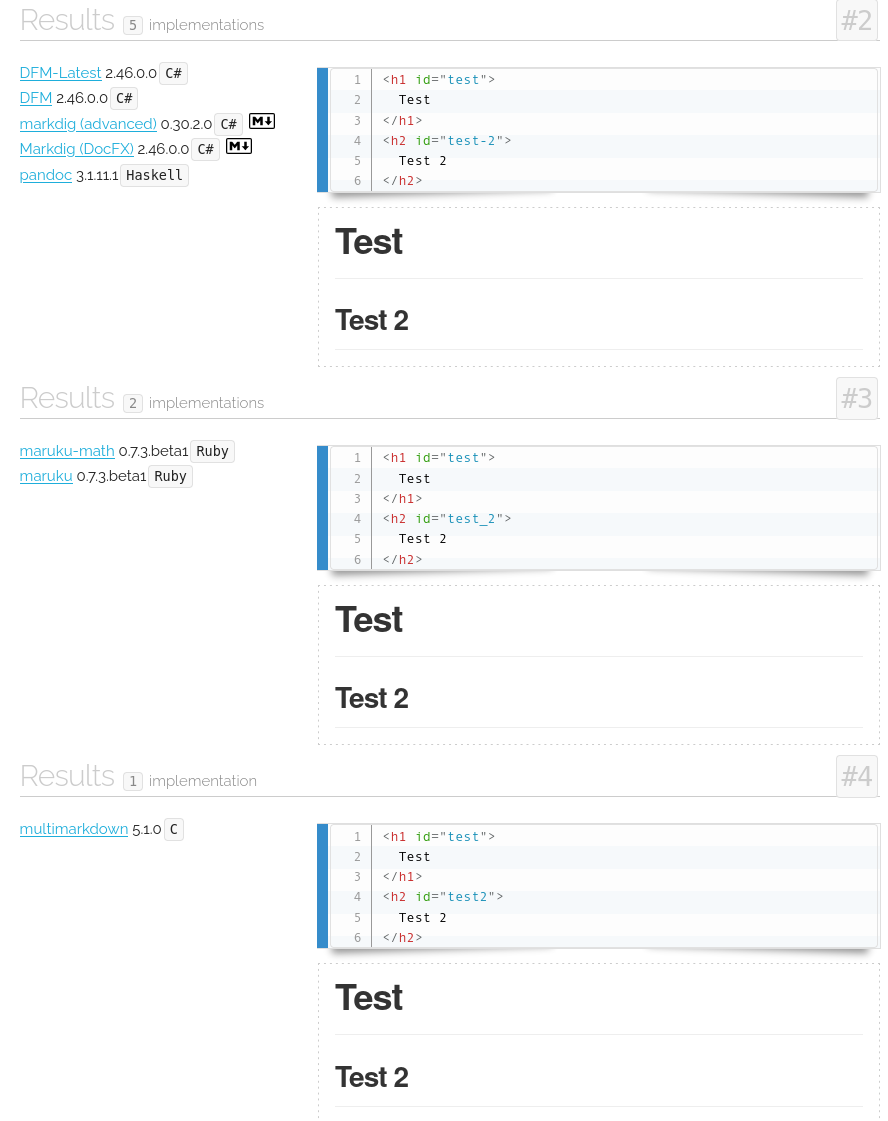
\includegraphics[scale=0.35]{babelmark}
\caption{Babelmark listing many possible HTML outputs}
\label{fig:babelmark}
\end{figure}

\section{Standardization efforts}

Frustrated by the multiplication of divergent implementations, a group of people tried to push for a standard specification of Markdown to be created.
In the words of their creators, CommonMark is a "standard, unambiguous syntax specification for Markdown, along with a suite of comprehensive tests to
validate Markdown implementations against this specification".\footcite{commonmark} This group, led by Pandoc's creator \citeauthor{pandoc}, has promised
for many years that they would deliver a finalized specification "soon", the last official communication giving a deadline in 2019.
So far, albeit quite a lot of work being achieved, a major version has yet to appear.

\section{Markdown ``flavours'' and their impact}

As seen in chapter \ref{chap:issues}, the qualities of Markdown outweighing its flaws, and opinionated people wanting to solve its issues
their own way, the proliferation of new syntaxes and interpreters that are supersets or modifications of the original syntax made their appearance,
which are commonly called ``Markdown flavours''. These allowed many tools and use-cases to come to life, by adding many features which go far
beyond simple document markup. In the following sub-sections, we'll explore how some of the missing features listed in section \ref{sec: missing-features}
were addressed by open source software creators, and how these tools impacted various fields or domains.

\subsection{Reproductible research}

The main impact of Markdown and its variants, in this article's author opinion, is reproductible research. Several tools have been created in order to help
researchers, teachers and students to craft elegant and self-contained research papers with a much lower learning curve than LaTeX would for the equivalent
document produced.\newline

The most famous package in this ecosystem of tools is RMarkdown. It is described as a combination of "knitr, pandoc and a range of packages that coexist
in the background to produce publication quality reproducible research"\footcite{racine2019energy}. This fusion of tools allows users to intertwine both
the text which will be the contents of the report, and the data + data analysis themselves. This means that, in the same document, users can describe
a chart just after writing the code which generates and displays it in the report. The reproducible aspect of it stems from the fact that, as long as
any other user willing to generate the same report has the data required to process it, anyone is able to generate the same report and modify it on the
fly. It is an extremely powerful concept, which if combined with code versioning tools allows researchers to collaborate on the same paper in a much more
efficient way.

\subsection{Book/Textbook creation}

Tools such as MdBook or Bookdown allow its users to create books in a very efficient way, through a set of Markdown files and metadata.
This proved extremely useful in contexts such as the COVID-19 epidemic, when universities were forced to transition a lot of their teaching
online. One such experiment proved successful in engaging students in a complex time, and was a very effective tool at a time where the study
materials needed to be created very fast. \citeauthor{dunn2022your} describes the approach as allowing "for instant updating of material and 
provides focussed URLs that educators can use to point students directly to specific learning outcomes".\footcite{dunn2022your}

\subsection{Documentation (of code or not)}

One ecosystem where Markdown has thrived since its inception is code repositories. The very readable format of it made it the perfect companion
to document code in a longer format than comments tangled in the code. It is no wonder, then, that websites which host millions of code repositories
like Gitlab or Github have created their own extensions to Markdown. Github's one, called GFM (Github flavored markdown) is quite famous, allowing
to reference open issues, pull requests, changes, or code snippets on the fly with very simple syntax.\newline

Another very famous project in this realm is MKDocs, which allows users to create efficient documentation websites, with several pages, for more public
and sizeable projects, with content being written in Markdown.\newline

Lastly, a recent trend in the world of startups has been to describe software architecture design decisions for posterity through a format called ADR
(Architectural Decision Records). Quite fast, a Markdown template and accompanying tools to create these records was created and
shared online.\footcite{kopp2018markdown}